\documentclass{scrartcl}			% defines the kind of document you want to produce

% Include different packages:
\usepackage[utf8x]{inputenc}
\usepackage[T1]{fontenc}
\usepackage{lmodern}
\usepackage[english]{babel}
\usepackage{amsmath}
\usepackage{graphicx}           	% include graphics
\usepackage{caption}	
\usepackage{subcaption}	 
\usepackage{hyperref}
\usepackage{epstopdf}
\usepackage{siunitx}
\usepackage{float}

\title{Neuroprothetics Exercise 8\\Noise Vocoder}
\author{ Laura Bielenberg }
\date{\today}

\begin{document} 					% Document begins here

\maketitle

The code used to generate the following plots has been written using Python 3.7. Please run the  script \texttt{code/exercise\_8.py} to execute the code related to this exercise.

\section{Noise vocoder with dynamic compression}

\subsection{Filtered noise}\label{sec:filtnoise}
The initial noise signal is generated from a zero-mean Gaussian distribution and has the same length $N$ as the audio input array. Thus each sample $x_i ... x_N$ of the noise signal follows:
\begin{equation}
	x_i \sim \mathcal{N}(0, 1) \text{ for } i \in \left\{1 .. N\right\} \, .
\end{equation}
The noise signal is afterwards band-pass filtered by applying the CI filter banks from exercise 7.
Figure~\ref{fig:noise} shows the filtered noise for a 12 channel CI filter bank.

\begin{figure}[H]
\centering
   		 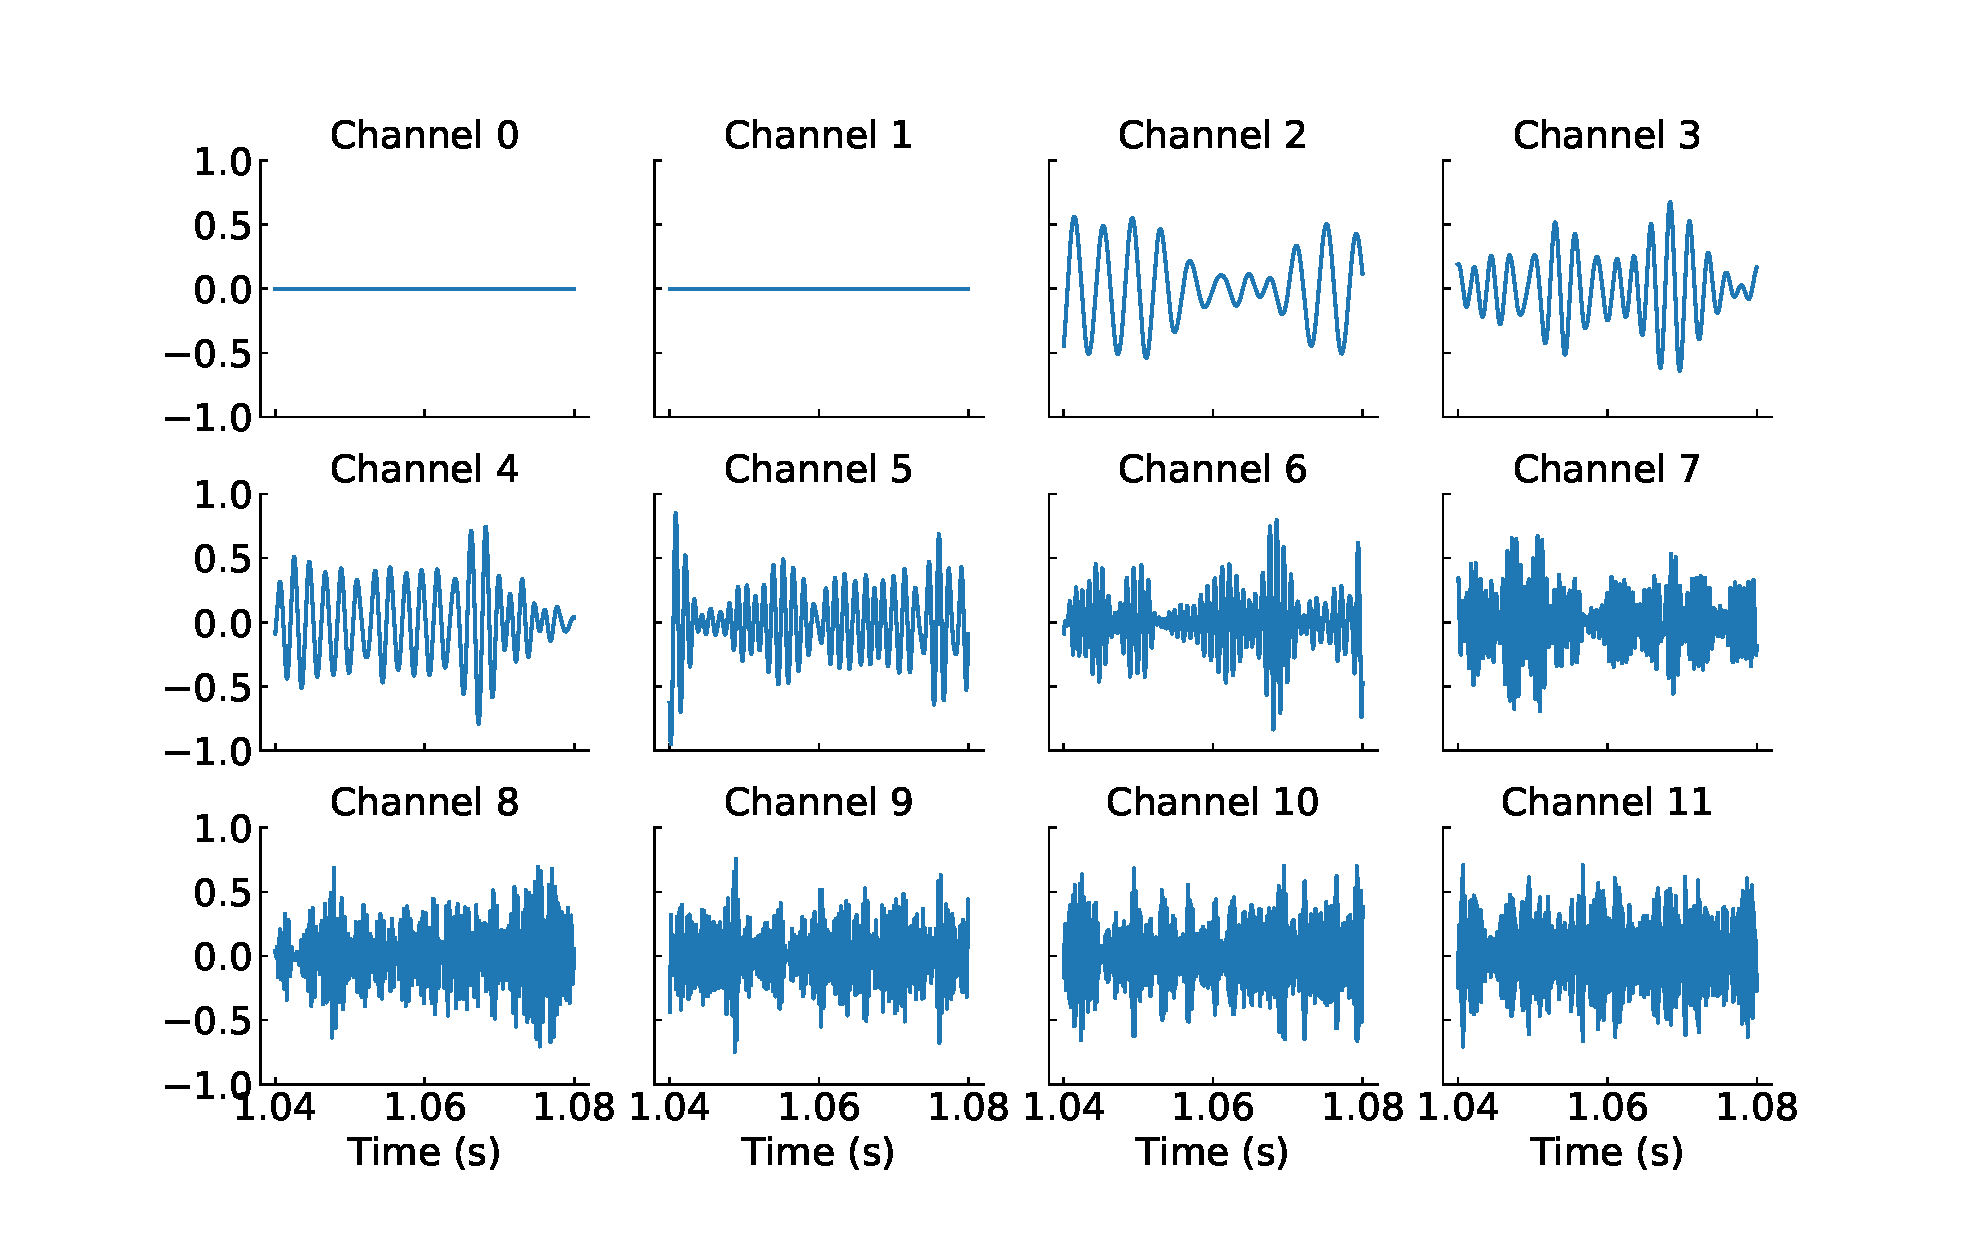
\includegraphics[width=\linewidth]{imgs/noise_filtered_timeslot.eps}
   		 \caption{Noise filtered by 12 CI filter bank.} 
   		 \label{fig:noise} 


\end{figure}

\subsection{Extract envelopes}
\begin{figure}[H]
\centering
   		 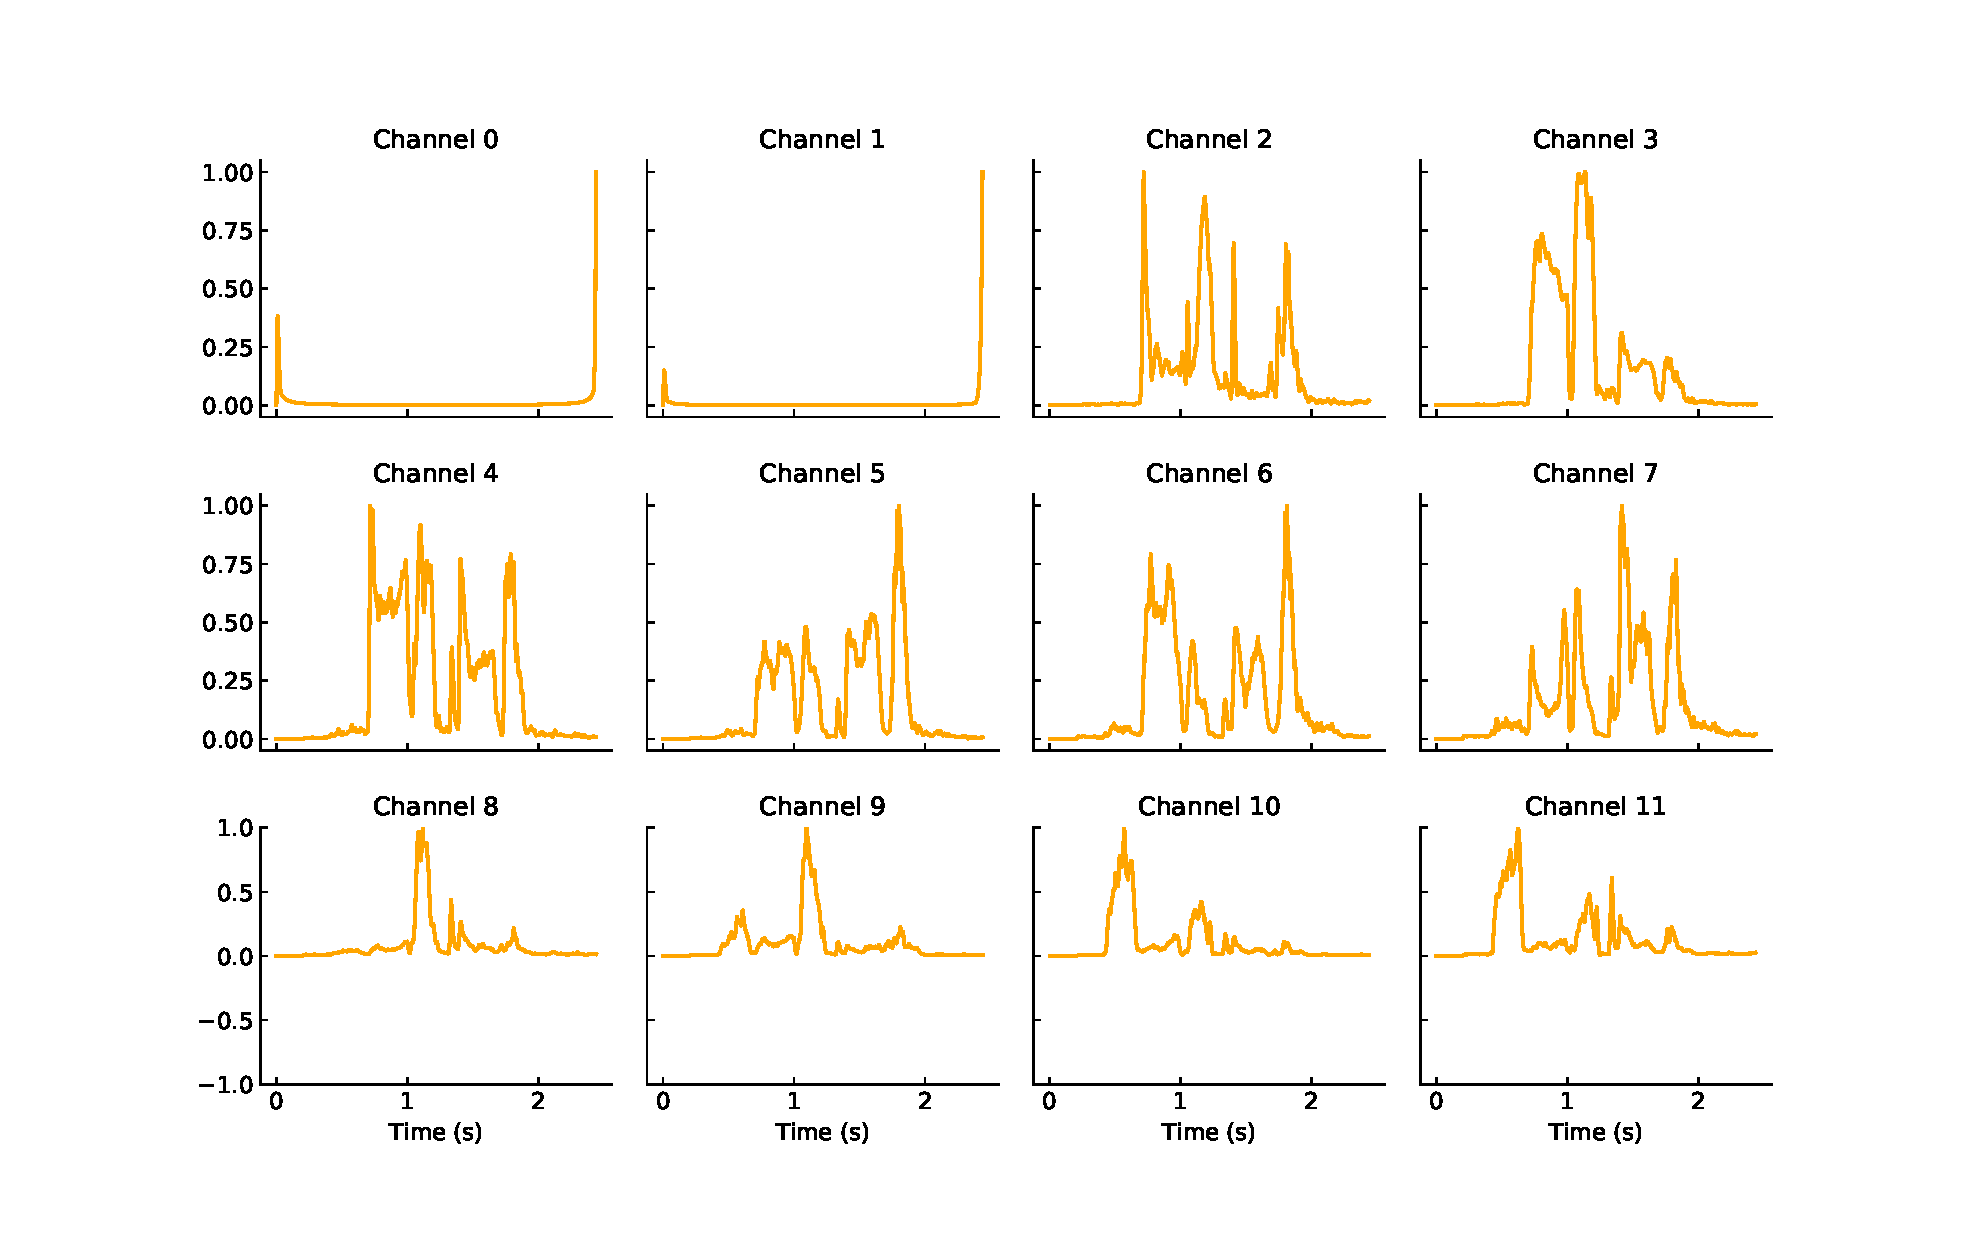
\includegraphics[width=\linewidth]{imgs/envelopes.eps}
   		 \caption{Spectogram for a 12 electrode CI from exercise 7.} 
   		 \label{fig:ci_3} 
\end{figure}

\subsection{Add dynamic compression}
\begin{figure}[H]
\centering
   		 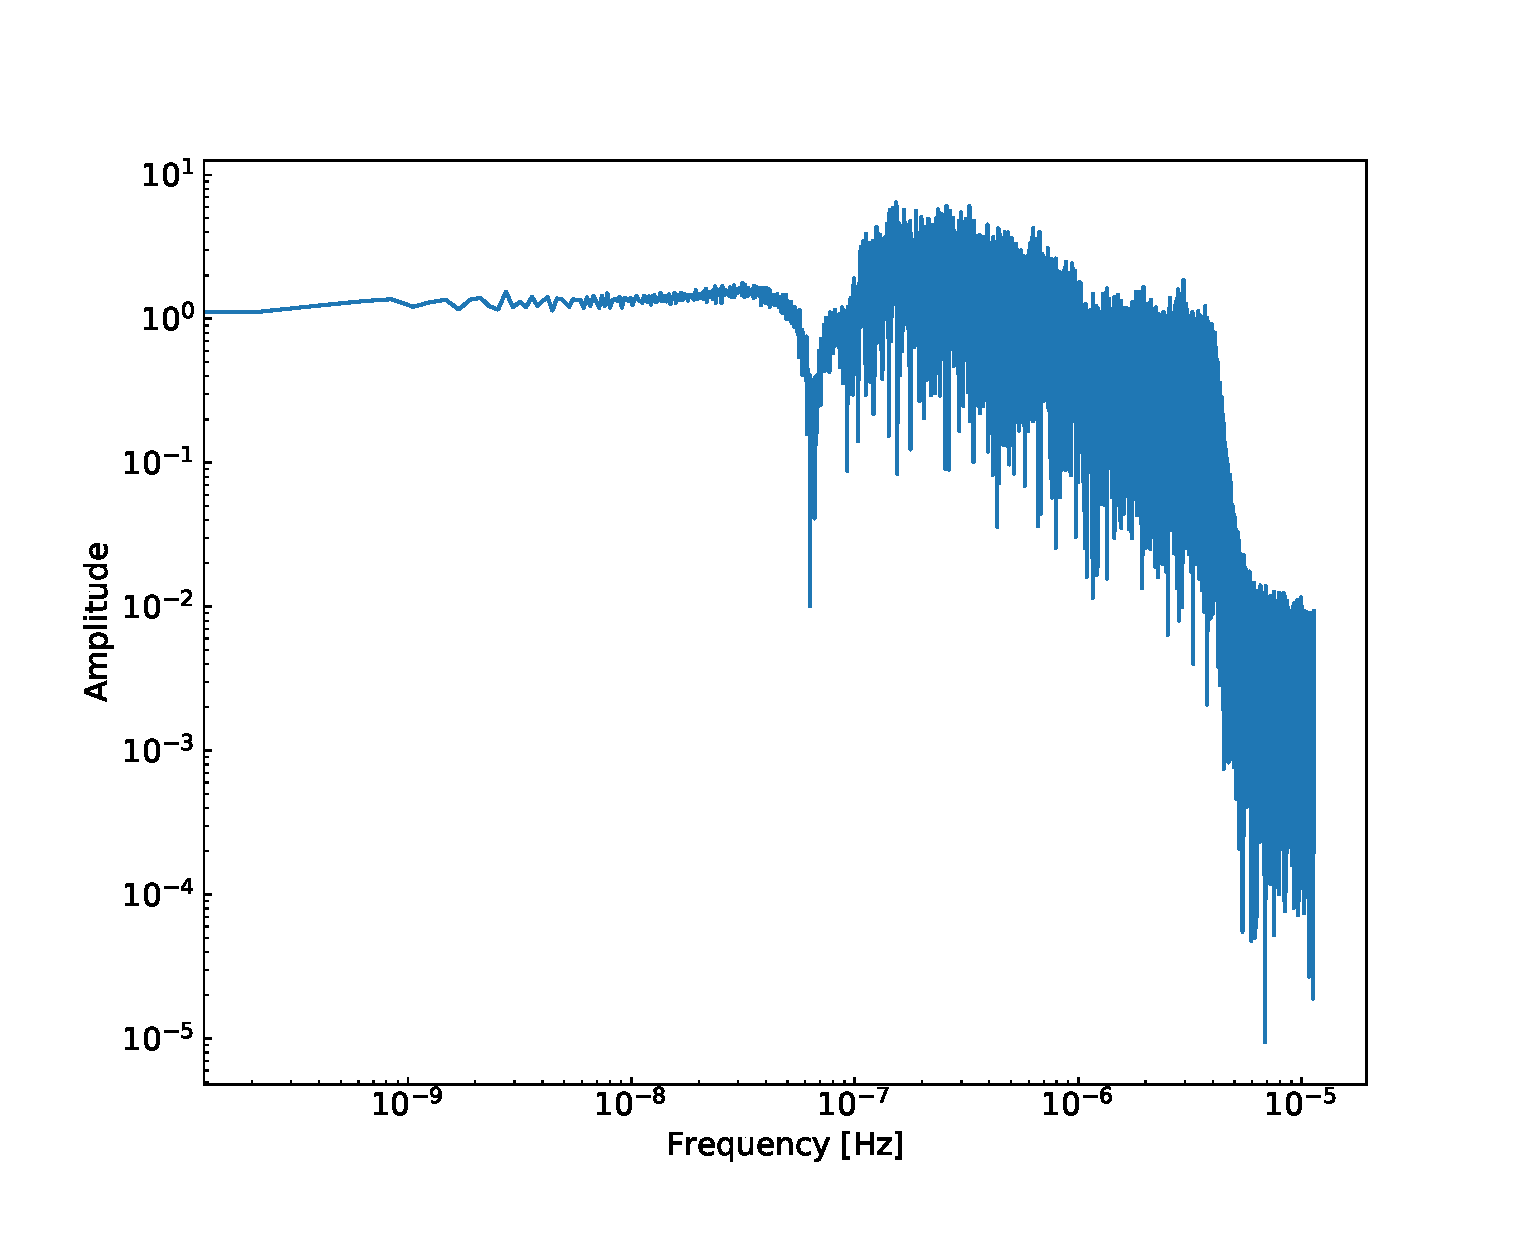
\includegraphics[width=0.8\linewidth]{imgs/vocoder_lower_clip_06.eps}
   		 \caption{Spectogram for a 12 electrode CI from exercise 7.} 
   		 \label{fig:ci_3} 
\end{figure}

\subsection{Finalize the Vocoder}
\begin{figure}[H]
\centering
   		 \includegraphics[width=\linewidth]{../tex_7/imgs/spectogram_12_CI.eps}
   		 \caption{Spectogram for a 12 electrode CI from exercise 7.} 
   		 \label{fig:ci_3} 


\end{figure}

\end{document}
